\section{Redes neurais convolucionais}
\label{sec:cnn}
\index{Redes neurais convolucionais}
\index{CNN}
\index{RNC}

Redes neurais convolucionais foram desenvolvidas para resolver o problema de aprender o relacionamento entre dados adjacentes e são amplamente utilizadas para o processamento de imagens justamente por terem a capacidade de extrair características uteis para reconhecimento de objetos e classificação \cite{zhang_dive_2021}. Este modelo possui inspiração na biologia, teoria de grupos entre outros \cite{zhang_dive_2021}. Nesta seção as redes neurais convolucionais serão introduzidas.

Convolução é um conceito matemático que é calculado entre duas funções \textit{f} e \textit{g} e mede o quanto a função \textit{g} se sobrepõe à função \textit{f} se \textit{g} se desloca através de \textit{f} e é calculada formalmente como \cite{wikipedia_convolucao_2020, weisstein_convolution_2003, zhang_dive_2021}:

\begin{equation}
    (f * g)(x) = \int f(z)g(x-z)dz
    \label{eq:eq1}
\end{equation}

A equação \ref{eq:eq1} pode ser generalizada para múltiplas dimensões, como é o caso de imagens. Imagens em preto e branco podem ser definidas com duas dimensões (largura e altura) enquanto imagens coloridas podem ser definidas com três dimensões (largura, altura e cor). 

Para detectar um objeto em específico em uma imagem, considerando que o modelo matemático desta esteja disponível, pode-se calcular a convolução da primeira imagem em relação ao objeto. Assim, os pontos mais propensos de se encontrar o objeto terão um pico na convolução \cite{zhang_dive_2021}. No caso de imagens coloridas, essas convoluções devem ser adaptadas para trabalhar com canais de cores diferentes (vermelho, verde e azul): os três canais que compõem uma imagem colorida. As convoluções extraem características da imagem e reduzem a complexidade do processamento. De acordo com \cite{zhang_dive_2021}, camadas de convoluções geralmente requerem menos parâmetros que uma rede completamente conectada, como um MLP. \index{MLP} \index{Multilayer Perceptron}

Para capturar detalhes espaciais de uma imagem, as redes convolucionais conectam um conjunto de pixels adjacentes em um único neurônio da próxima camada. Este neurônio tem um nome especial. É conhecido como \textit{campo receptivo local}. Esta operação que acaba de ser descrita é uma convolução \cite{gulli_deep_2019}. Veja a imagem abaixo:

\begin{figure}[H]
    \centering
    \caption{Exemplo de operação de convolução. Os números foram propositalmente colocados de forma repetitiva para facilitar a explicação e os cálculos.}
    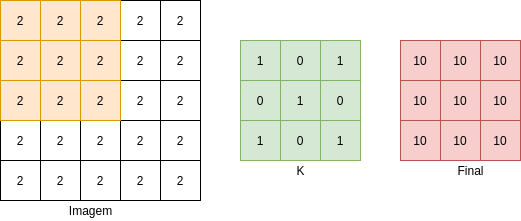
\includegraphics[width=12cm]{fig/conv.png}
    \legend{Fonte: autor, baseado em \cite{zhang_dive_2021}}
    \label{fig:fig4}
\end{figure}

Na figura \ref{fig:fig4}, a matriz de entrada representa uma imagem e a matriz \textit{K} é a matriz com a qual iremos fazer a convolução da imagem. Em redes convolucionais (chamaremos de CNN a partir de agora para sermos mais breve. CNN vem do inglês, \textit{convolutional neural networks} que traduz diretamente para redes neurais convolucionais), essa matriz \textit{K} é chamada de \textit{kernel} ou \textit{núcleo}, em português. Esta matriz é responsável por extrair informações da imagem. No exemplo anterior, da figura \ref{fig:fig4}, durante cada iteração da convolução, sobrepõe-se um subconjunto de pixels da imagem. Na primeira iteração, ela sobrepõe os pixels pintados em amarelo e o resultado desta convolução é 10 (2*1 + 2*0 + 2*1 + 2*0 + 2*1 + 2*0 + 2*1 + 2*0 + 2*1 = 10), portanto, na próxima camada, temos uma saída no valor de 10. Na próxima iteração, a matriz núcleo se desloca em um pixel para a direita e faz a mesma operação. Quando ela atinge o final da matriz de imagem, volta ao início e desloca um pixel abaixo, e assim por diante até cobrir toda a imagem. Por meio dessas operações, somos capazes de aproveitar e aprender o relacionamento entre pixels adjacentes, algo que não é tão simples de se fazer com uma rede MLP.

Além de convoluções, uma funcionalidade importante em redes convolucionais, é o \textit{pooling}. Esta operação reduz a complexidade e a resolução das características agregadas e aprendendidas de uma imagem a medida que o processamento da imagem acontece. No final das contas, o objetivo é capturar detalhes específicos da imagem. Estes detalhes, devem ser suficientes para se extrair a informação necessária. Identificar um objeto em uma imagem como um cachorro, uma pessoa, um carro etc. por exemplo. As ultimas camadas da rede devem ser bastante sensíveis à imagem de entrada, de forma que se a alterarmos minimamente, a alteração trará consequências significativas ao resultado final. A saída de uma camada de convolução é chamada de \textit{feature map} (mapa de atributos, do inglês) \cite{zhang_dive_2021, brownlee_gentle_nodate}. 

Existem várias formas de se fazer o \textit{pooling}, entre elas temos \textit{max pooling} e \textit{average pooling}.

\subsection{Max Pooling}

Para fazer o \textit{max pooling} de uma matriz, seleciona-se um subconjunto de seus pixels, representando-os como um único dado para a próxima camada: o pixel com o maior valor \cite{zhang_dive_2021, brownlee_gentle_nodate}. O diagrama abaixo (figura \ref{fig:fig5} ilustra de forma simplória a técnica de \textit{max pooling}. Da esquerda para direita, e cima para baixo a operação opera sobre toda a matriz. Percebe-se que alguns valores aprecem mais vezes. Talvez reduzir o tamanho da matriz de \textit{pooling} (conhecida também como janela de \textit{pooling}) ou normalizar os \textit{pixels} da imagem antes do processamento, seja uma forma de evitar tais repetições excessivas.

\begin{figure}[H]
    \centering
    \caption{Exemplo de operação de \textit{max pooling}.}
    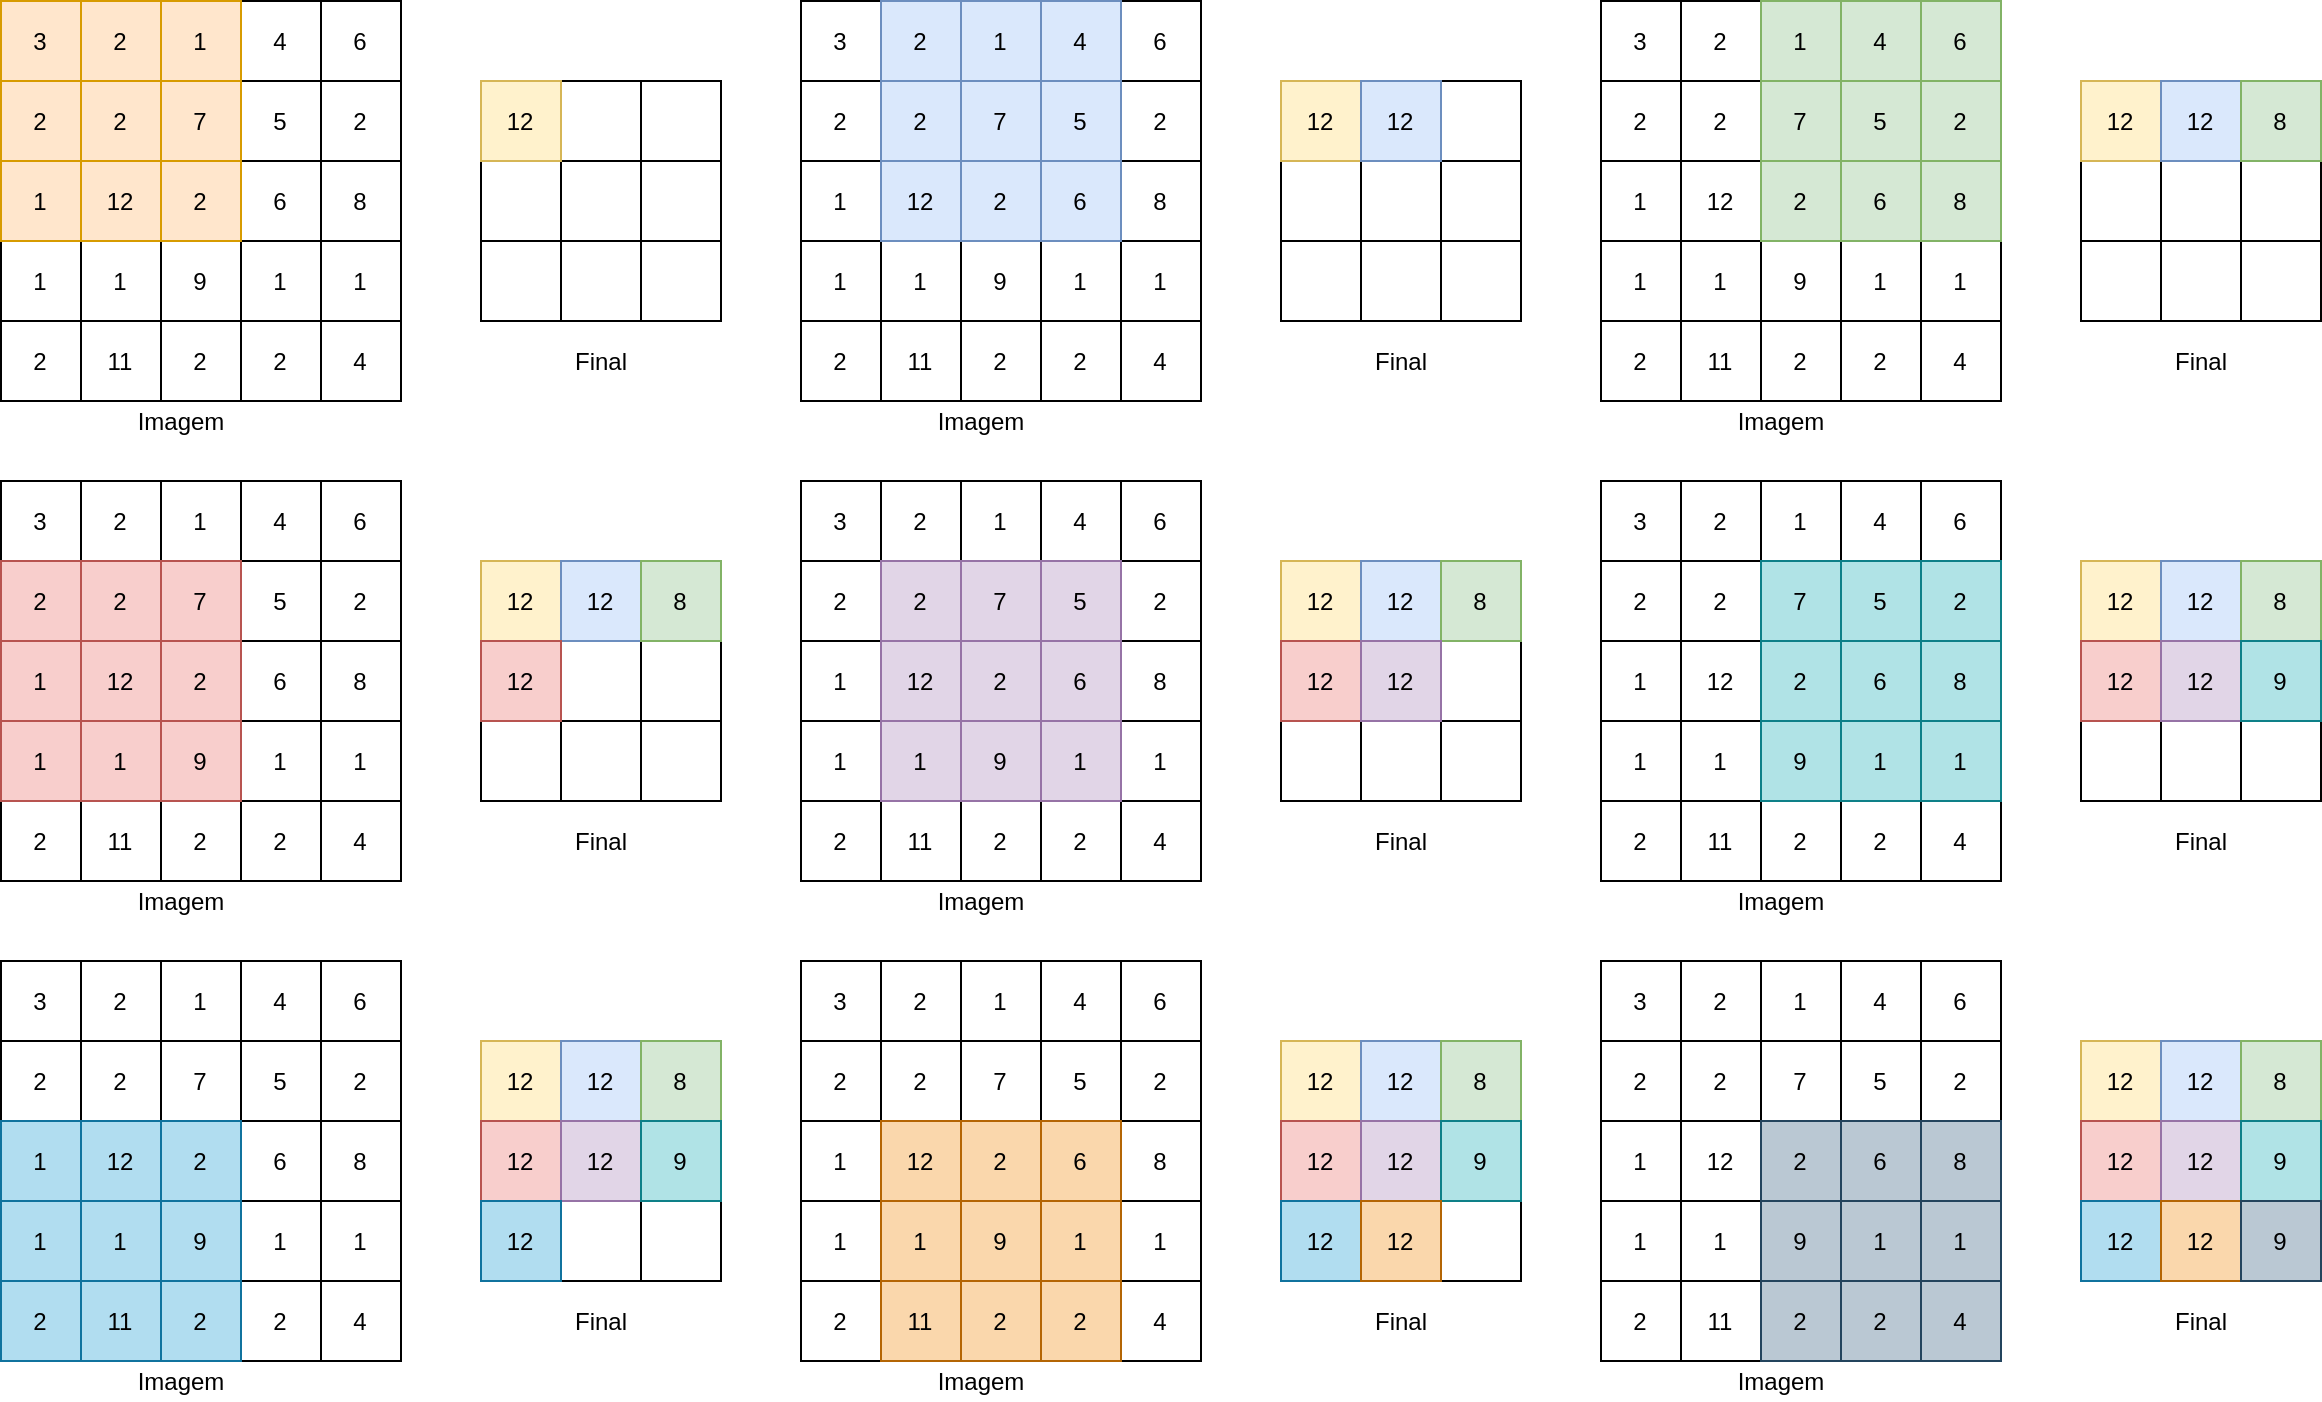
\includegraphics[width=13cm]{fig/Max Pooling.png}
    \legend{Fonte: autor, baseado em \cite{zhang_dive_2021, gulli_deep_2019}}
    \label{fig:fig5}
\end{figure}

\subsection{Average Pooling}

Esta operação é bastante parecida com o \textit{max pooling} na forma como é realizada, porém o cálculo é diferente. Em vez de se calcular o valor máximo dos pixels da matriz de entrada, calcula-se a média aritmética \cite{zhang_dive_2021, brownlee_gentle_nodate}. O diagrama abaixo ilustra o que foi dito:

\begin{figure}[H]
    \centering
    \caption{Exemplo de operação de \textit{average pooling}. Da esquerda para direita, e cima para baixo a operação é realizada sobre toda a matriz.}
    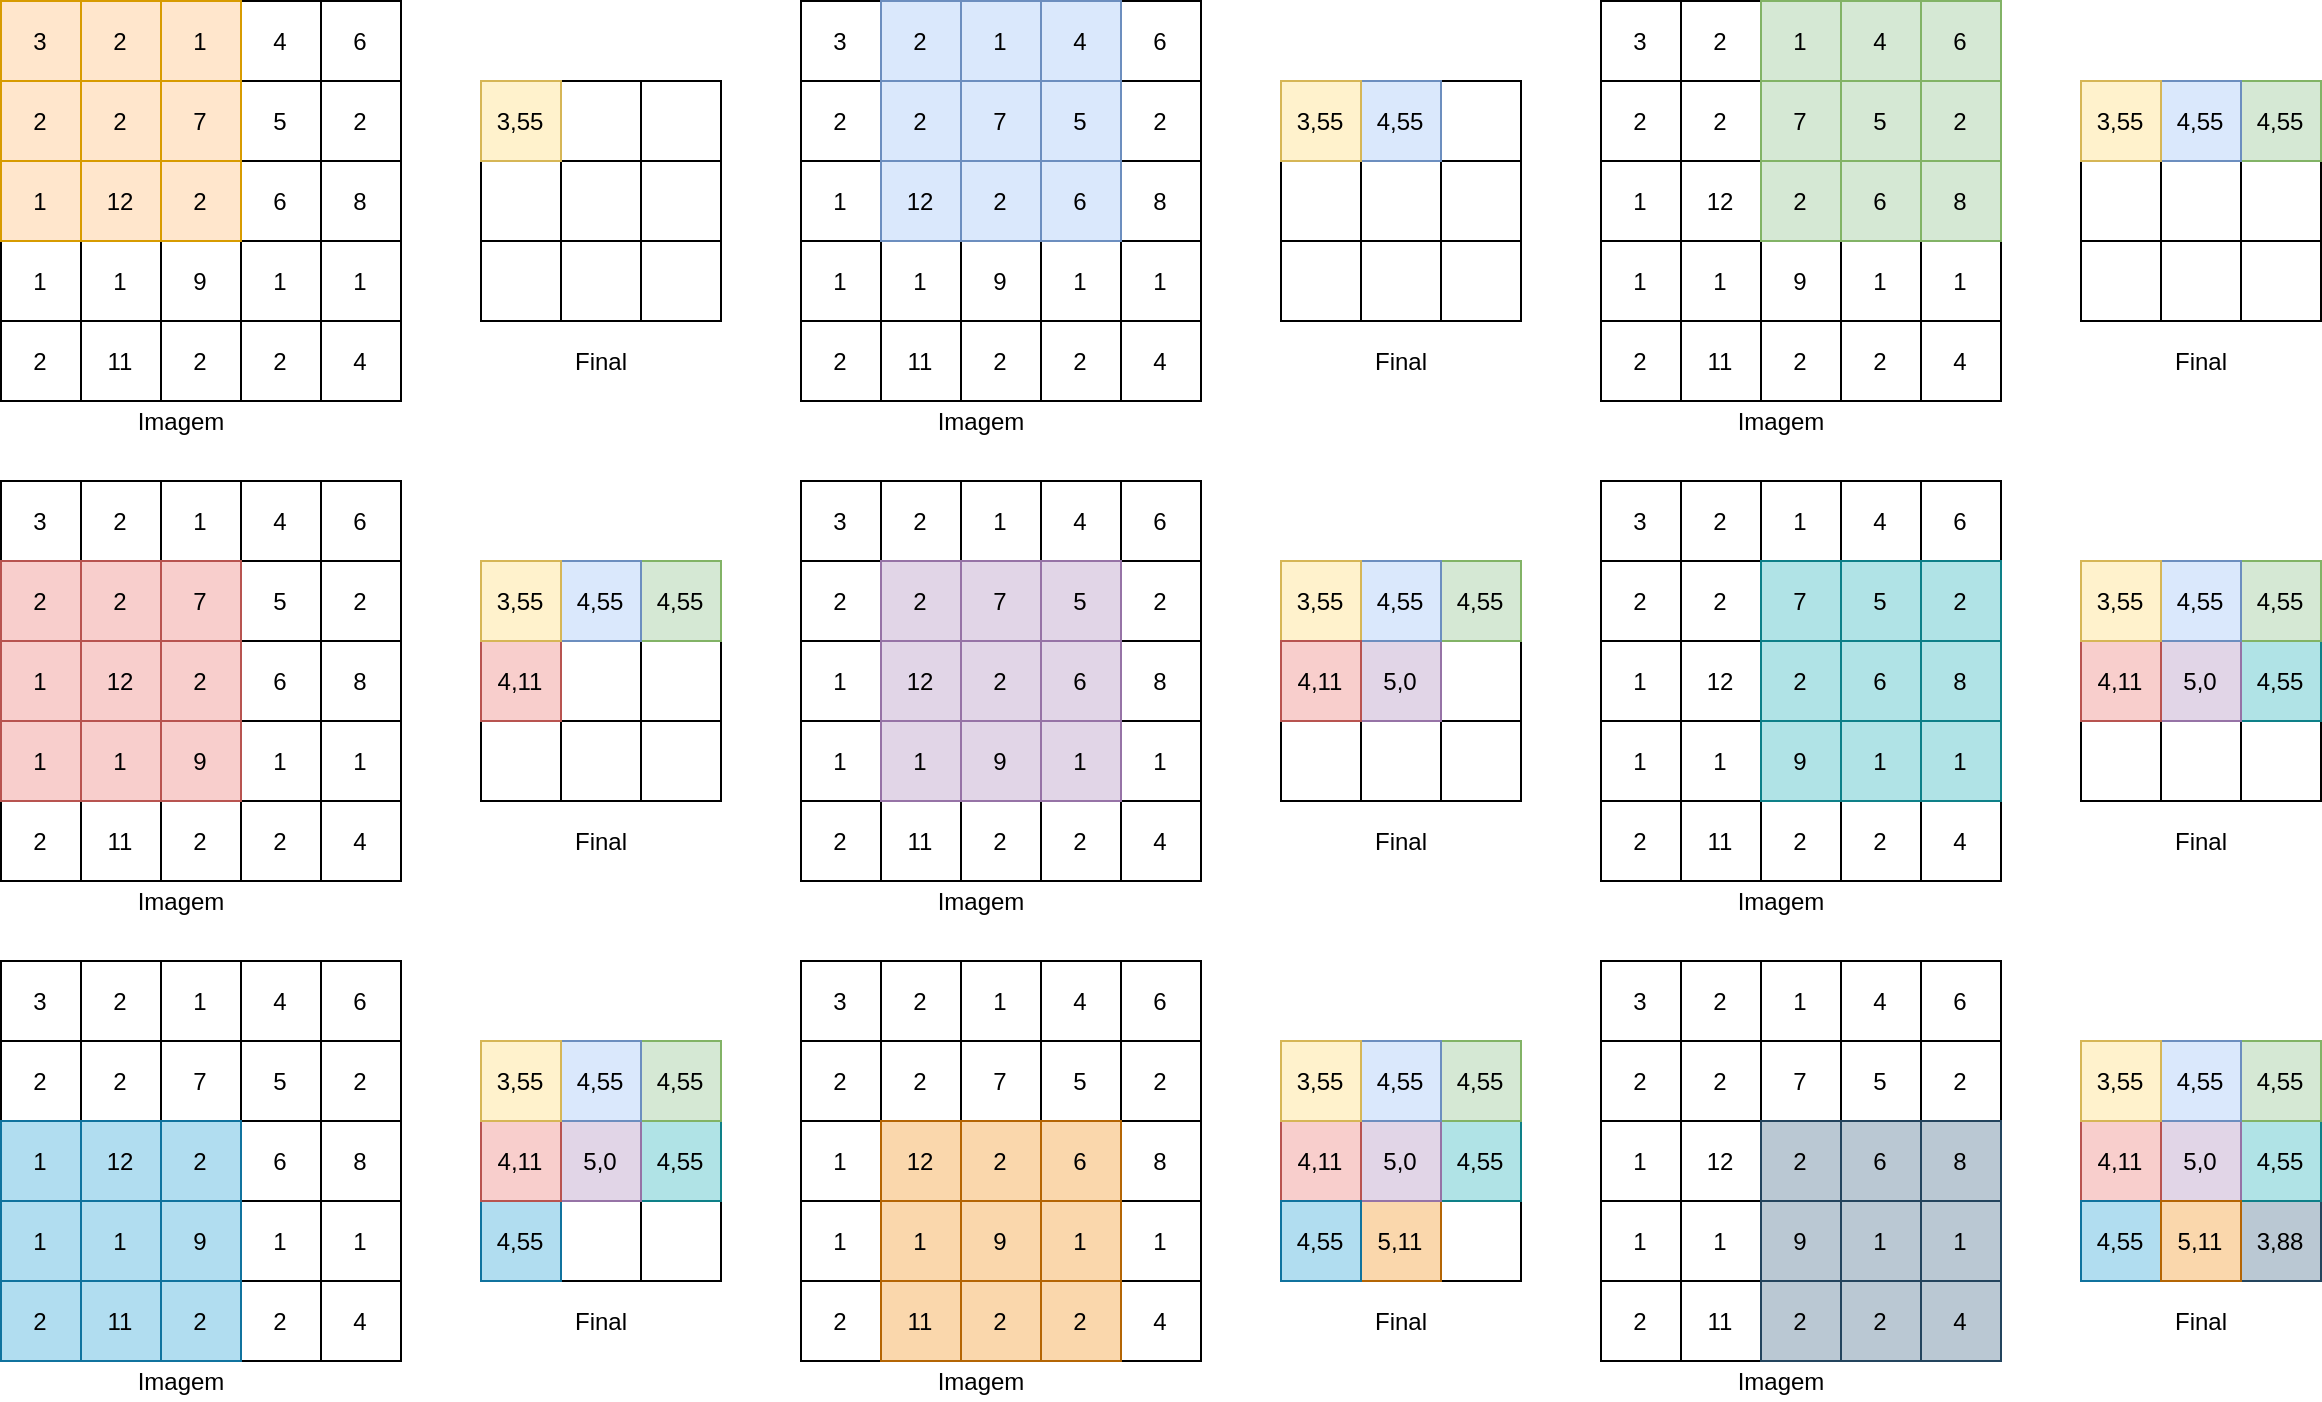
\includegraphics[width=13cm]{fig/Avg Pooling.png}
    \legend{Fonte: autor, baseado em \cite{zhang_dive_2021, gulli_deep_2019}.}
    \label{fig:fig6}
\end{figure}

\subsection{A arquitetura da rede}

Redes convolucionais podem ser organizadas das mais variadas maneiras existentes para as mais variadas tarefas. Duas formas famosas na literatura, são as redes convolucionais para classificação que terminam completamente conectadas e as completamente convolucionais. A primeira arquitetura consiste em uma CNN tradicional, com as camadas de convolução e \textit{pooling}, porém no final ela se conecta a uma rede completamente conectada (i.e. cada neurônio da camada anterior se conecta a todos neurônios da próxima camada) como um MLP e a partir dele pode classificar o conteúdo de uma imagem, como o exemplo famoso de detectar se o objeto da foto é um cachorro ou um gato. Nesse caso, a CNN irá extrair das imagens as características necessárias para avaliar o que o objeto é. Com as características extraídas, estas são alimentadas na rede completamente conectada e esta por sua vez faz a classificação.

A segunda arquitetura não envolve camadas completamente conectadas. Neste modelo, a rede mantém a estrutura da CNN até a última camada. Um exemplo de aplicação desta arquitetura, é a segmentação de imagens. Aproveitando o caso de uso da arquitetura anterior, suponha que em vez de identificar se na imagem há um gato ou um cachorro, o objetivo seja descobrir onde especificamente, naquela imagem está o cachorro. Para esta funcionalidade, a rede precisaria de não apenas detectar as características da imagem e identificar o cachorro, como também precisaria demarcar o animal na imagem. Para isso, essas redes utilizam as características extraídas nas camadas iniciais para reconstruir a imagem nas camadas finais, destacando o objeto em questão \cite{kumar_semantic_2020}.

Para este trabalho, ambas as arquiteturas serão utilizadas. Nas próximas seções, ficará mais claro a aplicação de cada uma destas.
